\documentclass[a4paper,11pt]{book}\usepackage[]{graphicx}\usepackage[]{color}
%% maxwidth is the original width if it is less than linewidth
%% otherwise use linewidth (to make sure the graphics do not exceed the margin)
\makeatletter
\def\maxwidth{ %
  \ifdim\Gin@nat@width>\linewidth
    \linewidth
  \else
    \Gin@nat@width
  \fi
}
\makeatother

\definecolor{fgcolor}{rgb}{0.345, 0.345, 0.345}
\newcommand{\hlnum}[1]{\textcolor[rgb]{0.686,0.059,0.569}{#1}}%
\newcommand{\hlstr}[1]{\textcolor[rgb]{0.192,0.494,0.8}{#1}}%
\newcommand{\hlcom}[1]{\textcolor[rgb]{0.678,0.584,0.686}{\textit{#1}}}%
\newcommand{\hlopt}[1]{\textcolor[rgb]{0,0,0}{#1}}%
\newcommand{\hlstd}[1]{\textcolor[rgb]{0.345,0.345,0.345}{#1}}%
\newcommand{\hlkwa}[1]{\textcolor[rgb]{0.161,0.373,0.58}{\textbf{#1}}}%
\newcommand{\hlkwb}[1]{\textcolor[rgb]{0.69,0.353,0.396}{#1}}%
\newcommand{\hlkwc}[1]{\textcolor[rgb]{0.333,0.667,0.333}{#1}}%
\newcommand{\hlkwd}[1]{\textcolor[rgb]{0.737,0.353,0.396}{\textbf{#1}}}%

\usepackage{framed}
\makeatletter
\newenvironment{kframe}{%
 \def\at@end@of@kframe{}%
 \ifinner\ifhmode%
  \def\at@end@of@kframe{\end{minipage}}%
  \begin{minipage}{\columnwidth}%
 \fi\fi%
 \def\FrameCommand##1{\hskip\@totalleftmargin \hskip-\fboxsep
 \colorbox{shadecolor}{##1}\hskip-\fboxsep
     % There is no \\@totalrightmargin, so:
     \hskip-\linewidth \hskip-\@totalleftmargin \hskip\columnwidth}%
 \MakeFramed {\advance\hsize-\width
   \@totalleftmargin\z@ \linewidth\hsize
   \@setminipage}}%
 {\par\unskip\endMakeFramed%
 \at@end@of@kframe}
\makeatother

\definecolor{shadecolor}{rgb}{.97, .97, .97}
\definecolor{messagecolor}{rgb}{0, 0, 0}
\definecolor{warningcolor}{rgb}{1, 0, 1}
\definecolor{errorcolor}{rgb}{1, 0, 0}
\newenvironment{knitrout}{}{} % an empty environment to be redefined in TeX

\usepackage{alltt}
%\documentclass[a4paper,twoside,11pt,titlepage]{book}
\usepackage{listings}
\usepackage[utf8]{inputenc}
\usepackage[spanish]{babel}
\usepackage{float}

% \usepackage[style=list, number=none]{glossary} %
%\usepackage{titlesec}
%\usepackage{pailatino}

\decimalpoint
\usepackage{dcolumn}
\newcolumntype{.}{D{.}{\esperiod}{-1}}
\makeatletter
\addto\shorthandsspanish{\let\esperiod\es@period@code}
\makeatother


%\usepackage[chapter]{algorithm}
\RequirePackage{verbatim}
%\RequirePackage[Glenn]{fncychap}
\usepackage{fancyhdr}
\usepackage{graphicx}
\usepackage{afterpage}

\usepackage{longtable}

\usepackage[pdfborder={000}]{hyperref} %referencia

% ********************************************************************
% Re-usable information
% ********************************************************************
\newcommand{\myTitle}{Título del proyecto\xspace}
\newcommand{\myDegree}{Grado en ...\xspace}
\newcommand{\myName}{Nombre Apllido1 Apellido2 (alumno)\xspace}
\newcommand{\myProf}{Nombre Apllido1 Apellido2 (tutor1)\xspace}
\newcommand{\myOtherProf}{Nombre Apllido1 Apellido2 (tutor2)\xspace}
%\newcommand{\mySupervisor}{Put name here\xspace}
\newcommand{\myFaculty}{Escuela Técnica Superior de Ingenierías Informática y de
Telecomunicación\xspace}
\newcommand{\myFacultyShort}{E.T.S. de Ingenierías Informática y de
Telecomunicación\xspace}
\newcommand{\myDepartment}{Departamento de ...\xspace}
\newcommand{\myUni}{\protect{Universidad de Granada}\xspace}
\newcommand{\myLocation}{Granada\xspace}
\newcommand{\myTime}{\today\xspace}
\newcommand{\myVersion}{Version 0.1\xspace}


\hypersetup{
pdfauthor = {\myName (email (en) ugr (punto) es)},
pdftitle = {\myTitle},
pdfsubject = {},
pdfkeywords = {palabra_clave1, palabra_clave2, palabra_clave3, ...},
pdfcreator = {LaTeX con el paquete ....},
pdfproducer = {pdflatex}
}

%\hyphenation{}


%\usepackage{doxygen/doxygen}
%\usepackage{pdfpages}
\usepackage{url}
\usepackage{colortbl,longtable}
\usepackage[stable]{footmisc}
%\usepackage{index}

%\makeindex
%\usepackage[style=long, cols=2,border=plain,toc=true,number=none]{glossary}
% \makeglossary

% Definición de comandos que me son tiles:
%\renewcommand{\indexname}{Índice alfabético}
%\renewcommand{\glossaryname}{Glosario}

\pagestyle{fancy}
\fancyhf{}
\fancyhead[LO]{\leftmark}
\fancyhead[RE]{\rightmark}
\fancyhead[RO,LE]{\textbf{\thepage}}
\renewcommand{\chaptermark}[1]{\markboth{\textbf{#1}}{}}
\renewcommand{\sectionmark}[1]{\markright{\textbf{\thesection. #1}}}

\setlength{\headheight}{1.5\headheight}

\newcommand{\HRule}{\rule{\linewidth}{0.5mm}}
%Definimos los tipos teorema, ejemplo y definición podremos usar estos tipos
%simplemente poniendo \begin{teorema} \end{teorema} ...
\newtheorem{teorema}{Teorema}[chapter]
\newtheorem{ejemplo}{Ejemplo}[chapter]
\newtheorem{definicion}{Definición}[chapter]

\definecolor{gray97}{gray}{.97}
\definecolor{gray75}{gray}{.75}
\definecolor{gray45}{gray}{.45}
\definecolor{gray30}{gray}{.94}

\lstset{ frame=Ltb,
     framerule=0.5pt,
     aboveskip=0.5cm,
     framextopmargin=3pt,
     framexbottommargin=3pt,
     framexleftmargin=0.1cm,
     framesep=0pt,
     rulesep=.4pt,
     backgroundcolor=\color{gray97},
     rulesepcolor=\color{black},
     %
     stringstyle=\ttfamily,
     showstringspaces = false,
     basicstyle=\scriptsize\ttfamily,
     commentstyle=\color{gray45},
     keywordstyle=\bfseries,
     %
     numbers=left,
     numbersep=6pt,
     numberstyle=\tiny,
     numberfirstline = false,
     breaklines=true,
   }

% minimizar fragmentado de listados
\lstnewenvironment{listing}[1][]
   {\lstset{#1}\pagebreak[0]}{\pagebreak[0]}

\lstdefinestyle{CodigoC}
   {
	basicstyle=\scriptsize,
	frame=single,
	language=C,
	numbers=left
   }
\lstdefinestyle{CodigoC++}
   {
	basicstyle=\small,
	frame=single,
	backgroundcolor=\color{gray30},
	language=C++,
	numbers=left
   }


\lstdefinestyle{Consola}
   {basicstyle=\scriptsize\bf\ttfamily,
    backgroundcolor=\color{gray30},
    frame=single,
    numbers=none
   }


\newcommand{\bigrule}{\titlerule[0.5mm]}


%Para conseguir que en las páginas en blanco no ponga cabecerass
\makeatletter
\def\clearpage{%
  \ifvmode
    \ifnum \@dbltopnum =\m@ne
      \ifdim \pagetotal <\topskip
        \hbox{}
      \fi
    \fi
  \fi
  \newpage
  \thispagestyle{empty}
  \write\m@ne{}
  \vbox{}
  \penalty -\@Mi
}
\makeatother

\usepackage{pdfpages}
\usepackage[T1]{fontenc}
\IfFileExists{upquote.sty}{\usepackage{upquote}}{}
\begin{document}
%\SweaveOpts{concordance=TRUE}
%\begin{titlepage}
 
 
\newlength{\centeroffset}
\setlength{\centeroffset}{-0.5\oddsidemargin}
\addtolength{\centeroffset}{0.5\evensidemargin}
\thispagestyle{empty}

\noindent\hspace*{\centeroffset}\begin{minipage}{\textwidth}

\centering

\includegraphics[width=0.9\textwidth]{imagenes/logo_ugr.jpg}\\[1.4cm]

\textsc{ \Large TRABAJO FIN DE GRADO\\[0.2cm]}
\textsc{ INGENIERÍA EN ...}\\[1cm]
% Upper part of the page
% 
% Title
{\Huge\bfseries Titulo del Proyecto\\
}
\noindent\rule[-1ex]{\textwidth}{3pt}\\[3.5ex]
{\large\bfseries Subtitulo del Proyecto}
\end{minipage}

\vspace{2.5cm}
\noindent\hspace*{\centeroffset}\begin{minipage}{\textwidth}
\centering

\textbf{Autor}\\ {Nombre Apellido1 Apellido2 (alumno)}\\[2.5ex]
\textbf{Directores}\\
{Nombre Apellido1 Apellido2 (tutor1)\\
Nombre Apellido1 Apellido2 (tutor2)}\\[2cm]

\includegraphics[width=0.3\textwidth]{imagenes/etsiit_logo.png}\\[0.1cm]
\textsc{Escuela Técnica Superior de Ingenierías Informática y de Telecomunicación}\\
\textsc{---}\\
Granada, mes de 201
\end{minipage}
%\addtolength{\textwidth}{\centeroffset}
%\vspace{\stretch{2}}
\end{titlepage}



%\chapter*{}
%\thispagestyle{empty}
%\cleardoublepage

%\thispagestyle{empty}

% \begin{titlepage}
 
 
\setlength{\centeroffset}{-0.5\oddsidemargin}
\addtolength{\centeroffset}{0.5\evensidemargin}
\thispagestyle{empty}

\noindent\hspace*{\centeroffset}\begin{minipage}{\textwidth}

\centering
%
\includegraphics[width=0.9\textwidth]{imagenes/logo_ugr.jpg}\\[1.4cm]

%\textsc{ \Large PROYECTO FIN DE CARRERA\\[0.2cm]}
%\textsc{ INGENIERÍA EN INFORMÁTICA}\\[1cm]
% Upper part of the page
% 

 \vspace{3.3cm}

%si el proyecto tiene logo poner aquí

\includegraphics{imagenes/logo.png} 
 \vspace{0.5cm}

% Title

{\Huge\bfseries Título del proyecto\\
}
\noindent\rule[-1ex]{\textwidth}{3pt}\\[3.5ex]
{\large\bfseries Subtítulo del proyecto.\\[4cm]}
\end{minipage}

\vspace{2.5cm}
\noindent\hspace*{\centeroffset}\begin{minipage}{\textwidth}
\centering

\textbf{Autor}\\ {Nombre Apellido1 Apellido2 (alumno)}\\[2.5ex]
\textbf{Directores}\\
{Nombre Apellido1 Apellido2 (tutor1)\\
Nombre Apellido1 Apellido2 (tutor2)}\\[2cm]
%
\includegraphics[width=0.15\textwidth]{imagenes/tstc.png}\\[0.1cm]
%\textsc{Departamento de Teoría de la Señal, Telemática y Comunicaciones}\\
%\textsc{---}\\
%Granada, mes de 201
\end{minipage}
%\addtolength{\textwidth}{\centeroffset}
\vspace{\stretch{2}}

 
\end{titlepage}






\cleardoublepage
\thispagestyle{empty}

\begin{center}
{\large\bfseries Estudio de optimización con incertidumbre en juegos de estrategia}\\
\end{center}
\begin{center}
Antonio Álvarez Caballero \\
\end{center}

%\vspace{0.7cm}
\noindent{\textbf{Palabras clave}: Estrategia, incertidumbre, datos, aprendizaje, predicción, clasificación}\\

\vspace{0.7cm}
\noindent{\textbf{Resumen}}\\

En este trabajo se realiza un estudio de la incertidumbre que presentan juegos
de estrategia en tiempo real como StarCraft, utilizando técnicas estadísticas
y de aprendizaje. Así se consigue evaluar la incertidumbre
que presentan este tipo de problemas para, en un paso posterior de optimización,
poder tenerla en cuenta y poder desarrollar agentes que sean capaces de evaluar
esta incertidumbre y actuar o modificar su conducta según lo necesite.

Se demostrará cómo el tiempo transcurrido es relevante en cuanto a la cantidad
de incertidumbre que presenta cada una de las partidas, aunque también se
expondrá que no es el factor más determinante: la información que un jugador
puede sacar del otro será incluso más importante.

\cleardoublepage


\thispagestyle{empty}


\begin{center}
{\large\bfseries Optimization study with uncertainty in strategy games}\\
\end{center}
\begin{center}
Antonio Álvarez Caballero \\
\end{center}

%\vspace{0.7cm}
\noindent{\textbf{Keywords}: Strategy, uncertainty, data, learning, prediction, classification}\\

\vspace{0.7cm}
\noindent{\textbf{Abstract}}\\

\begin{otherlanguage}{british}

In this project, the uncertainty that Real Time Strategy games like StarCraft
present is studied, applying statistical and learning techniques.
With all of this, uncertainty can be evaluated for next optimizations,
and thus agents able to evaluate this uncertainty and modify its strategy could
be developed.

\subsubsection*{Statistical Learning}

Firstly, the concept of \emph{statistical learning} is defined. It is a branch
of Mathematics that aims to learn unknown functions from data using statistical
techniques. This type of learning can be modelled mathematically to solve a
large set of problems in Science, Engineering, Economy, etc.

In-sample error and out-sample error concepts are introduced and used
throughout the entire project. In-sample error measure the accuracy based on
points that are inside the input space. Out-sample error measure the accuracy
on unknown points.

Then, the feasibility of learning in finite hypothesis sets is proven, mainly
using Hoeffding’s results: deviation between in-sample and out-sample errors
can be bounded, but exists a big limitation in these results. A hypothesis
function is set beforehand, so the desviation will depends on the data set.

After that, generalizing to infinite hypothesis sets is needed. These are the
most common sets in real life. For this purpose, the works of Vapnik and
Chervonenkis are presented. Their work from the 60’s to the 90’s involved
investigating in order to prove generalization and performing further relevant
research for the statistical learning theory. Their most important work is the
Vapnik-Chervonenkis bound. It bounds the out-sample error with the in-sample
one and a penalty term. This bound relies on the Vapnik-Chervonenkis dimension
of the model: an integer that represents the maximum number of points that a
model can shatter.

Using the Vapnik-Chervonenkis bound it is possible to measure the sample complexity and the
model complexity. In addition, the test set is introduced and analyzed using
Hoeffding's inequality.

Furthermore, the bias-var analysis is introduced in this chapter.
It models the out-of-sample error using the bias and the variance of the model,
it is considerably useful to develop new learning techniques and prevent overfitting.
It exists two approaches to achieve this: reduce bias without increase variance,
which is so application-related, and reduce variance without increase bias,
which is solved with general techniques.

Overfitting is the main problem of learning. It occurs when in-sample error is
great, but it does not generalizes at all. This is due to the fact that the
model is too complex and able to fit the noise of the data, giving a final
hypothesis that is worse than a simpler one. There are two types of noise:
stochastic and deterministic. Stochastic is random noise, and deterministic
is the region that the final hypothesis can't fit.

Validation tries to estimate de out-sample error using a similar idea of the
test set.

To combat overfitting Regularization could be used. Basically it constraints
the algorithms to improve out-of-sample error instead of minimizing in-sample
one. These methods are usually heuristics so there is a bit of art in this
field. A classical method of regularization is weight-decay. It constraints
the range of the coefficients of a final hypothesis.

In this chapter, the validation concept and the cross-validation method for
estimating out-of sample error are explained.


Lastly, in the mathematical background, the ensemble methods for learning are
described. These methods combine weak learners (only slightly better than
throwing a coin) to produce strong learners. Gradient Boosting is the reference
in this project.

\subsubsection*{Study of the uncertainty}

When anyone has to solve a data science problem the first step is understanding
the data that could be obtained and the problem that will be solved. There are
six StarCraft replays relational databases with a substantial amount of data,
and thus the first step is understanding them and selecting a subset.

After that, the data have to be preprocessed in order to be able to work with
statistical software. Dumping from a database, extracting the important features
and organizing them are basically an art. Whoever handles the data best could
have an important advantage.

The next step is doing an Exploratory Data Analysis, since obtaining a general
vision of the data and their distribution is essential. R is used for the
analysis because it is a good reference in statistics software. Barplots and
time plots are good tools to handle these data, and they could give some ideas to
fight them. As the dataset is too large, these ideas involve calculating the
slope of the regression line for each feature and each player, and calculating
the Area Under Curve of the feature graphs.

Then, XGBoost, the library used in this project, is described. It is an open
source library that implements the Gradient Boosting algorithm in a definitely
efficient way. It is the state of the art in learning libraries and it has great
importance in Kaggle competitions. It is used in some companies as well.

It provides a very efficient and effective way to classify data with ensemble
learning, with regularization techniques and parallel approaches; hence,
it is rather fast and provides excellent results.

Lastly, the results of playing with the data are explained, and conclusions
will be presented in the last chapter.

\subsubsection*{Conclusions}

The main conclusion of this work is that the time is not the main feature to
predict uncertainty: observed values from one player to the other one are
more useful if a powerful prediction model is used.




\end{otherlanguage}


\chapter*{}
\thispagestyle{empty}

\noindent\rule[-1ex]{\textwidth}{2pt}\\[4.5ex]

Yo, \textbf{Antonio Álvarez Caballero}, alumno de la titulación Doble Grado en
Ingeniería Informática y Matemáticas de la \textbf{Escuela Técnica Superior
de Ingenierías Informática y de Telecomunicación} y de la \textbf{Facultad de Ciencias}
de la \textbf{Universidad de Granada}, con DNI 15457968J, autorizo la
ubicación de la siguiente copia de mi Trabajo Fin de Grado en la biblioteca de
ambos centros para que pueda ser consultada por las personas que lo deseen.

\vspace{6cm}

\noindent Fdo: Antonio Álvarez Caballero

\vspace{2cm}

\begin{flushright}
Granada a \_ de Julio de 2016.
\end{flushright}


\chapter*{}
\thispagestyle{empty}

\noindent\rule[-1ex]{\textwidth}{2pt}\\[4.5ex]

D. \textbf{Juan Julián Merelo Guervós}, Profesor del Departamento Arquitectura y Tecnología de Computadores de la Universidad de Granada.

\vspace{0.5cm}

\textbf{Informa:}

\vspace{0.5cm}

Que el presente trabajo, titulado \textit{\textbf{Estudio de optimización con incertidumbre en juegos de estrategia}},
ha sido realizado bajo su supervisión por \textbf{Antonio Álvarez Caballero}, y autoriza la defensa de dicho trabajo ante el tribunal
que corresponda.

\vspace{0.5cm}

Y para que conste, expide y firma el presente informe en Granada a \_ de Julio de 2016.

\vspace{1cm}

\textbf{El director:}

\vspace{5cm}

\noindent \textbf{Juan Julián Merelo Guervós}

\chapter*{Agradecimientos}
\thispagestyle{empty}

       \vspace{1cm}


Quería agradecer a la Universidad de Granada y a los profesores de ambas
titulaciones por darme la oportunidad de formarme con ellos. En especial, a mi
tutor JJ Merelo por la oportunidad de realizar este trabajo y su ayuda durante
el transcurso del proyecto.

También agradecer a mi familia, sin cuyo apoyo constante no podría haber llegado
hasta aquí.

A mis amigos, sin cuya ayuda no habría sobrevivido a más de una asignatura.

A mi pareja, sin cuyo infinito apoyo no habría conseguido llegar hasta el final.

%\frontmatter
\tableofcontents
%\listoffigures
%\listoftables
%
%\mainmatter
%\setlength{\parskip}{5pt}




\chapter{Resumen}


\chapter{Abstract}


\chapter{Introducción}
% El primer paso es motivar el estudio del problema. Tienes que decir
% por qué te has decidido a hacer el TFM sobre eso y qué importancia
% puede tener en su contexto: IA en juegos, por ejemplo.


Probando

\begin{knitrout}
\definecolor{shadecolor}{rgb}{0.969, 0.969, 0.969}\color{fgcolor}\begin{figure}

{\centering 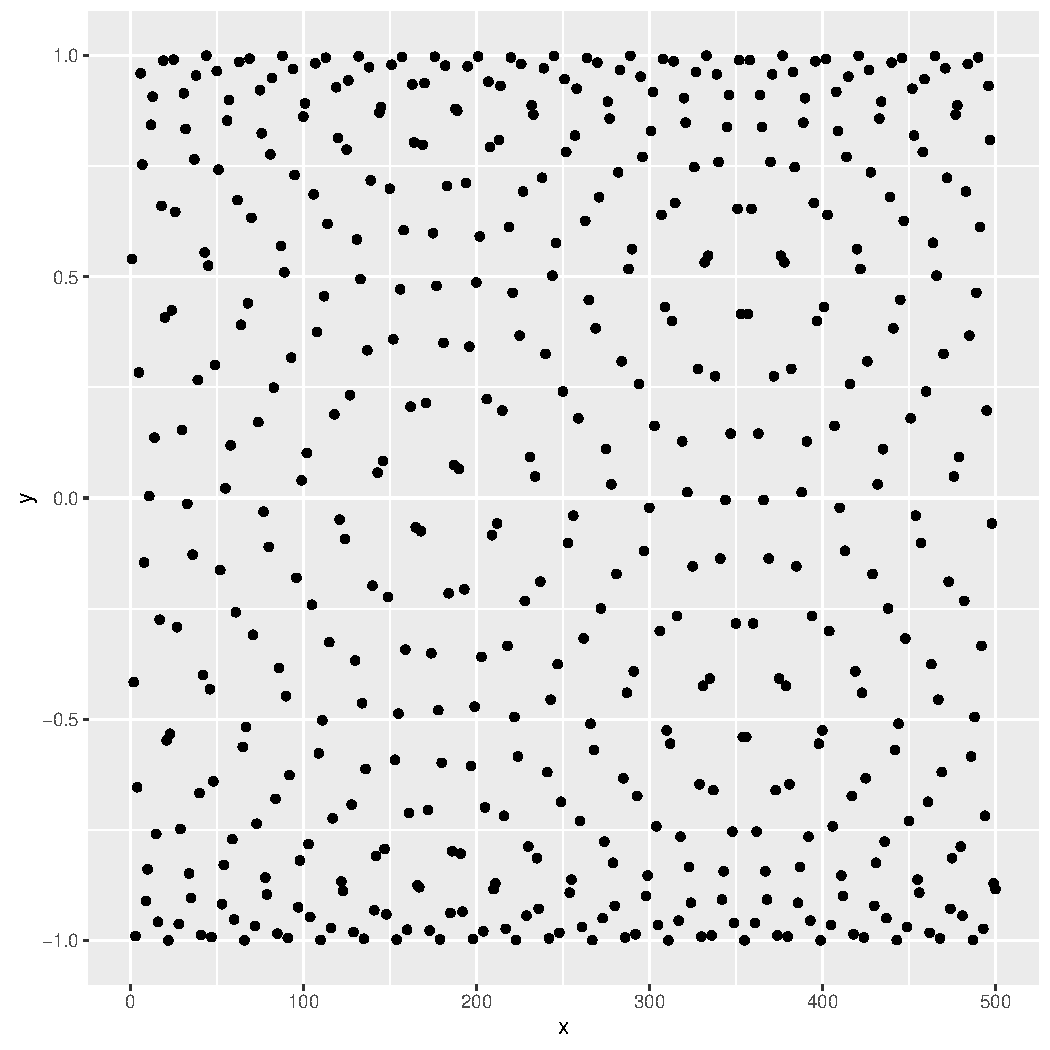
\includegraphics[width=\maxwidth]{figure/prueba-1} 

}

\caption[prueba]{prueba}\label{fig:prueba}
\end{figure}


\end{knitrout}

Prueba terminada~\ref{fig:prueba}


\chapter{Objetivos} 


\chapter{Desarrollo}


Introducción

\section{Matemáticas}
\label{sec:matematicas}
Aquí Mates

\section{Ingeniería Informática}
\label{sec:informatica}
Una vez se dispone de todas las herramientas matemáticas necesarias,
se puede comenzar con el desarrollo de la parte de Ingeniería Informática que
se aborda en el trabajo.

\subsection{Comprensión del problema y de los datos}
\label{subsec:comprension}

En primer lugar en cualquier problema de Ciencia de Datos, el primer
paso es \emph{comprender el problema y los datos que se disponen}.

El problema a abordar es el siguiente: a partir de un conjunto de
partidas antiguas de StarCraft~\cite{dataset2014}, se busca predecir
el momento en el que la partida está decidida con una confianza
determinada. Para ello, partimos de 6 bases de datos relacionales
(SQL) con gran cantidad de partidas almacenadas, cada una con muchas
características a observar. Cada una de ellas posee las
características presentes en la figura~\ref{dataset}.


\begin{figure}
    \centering
    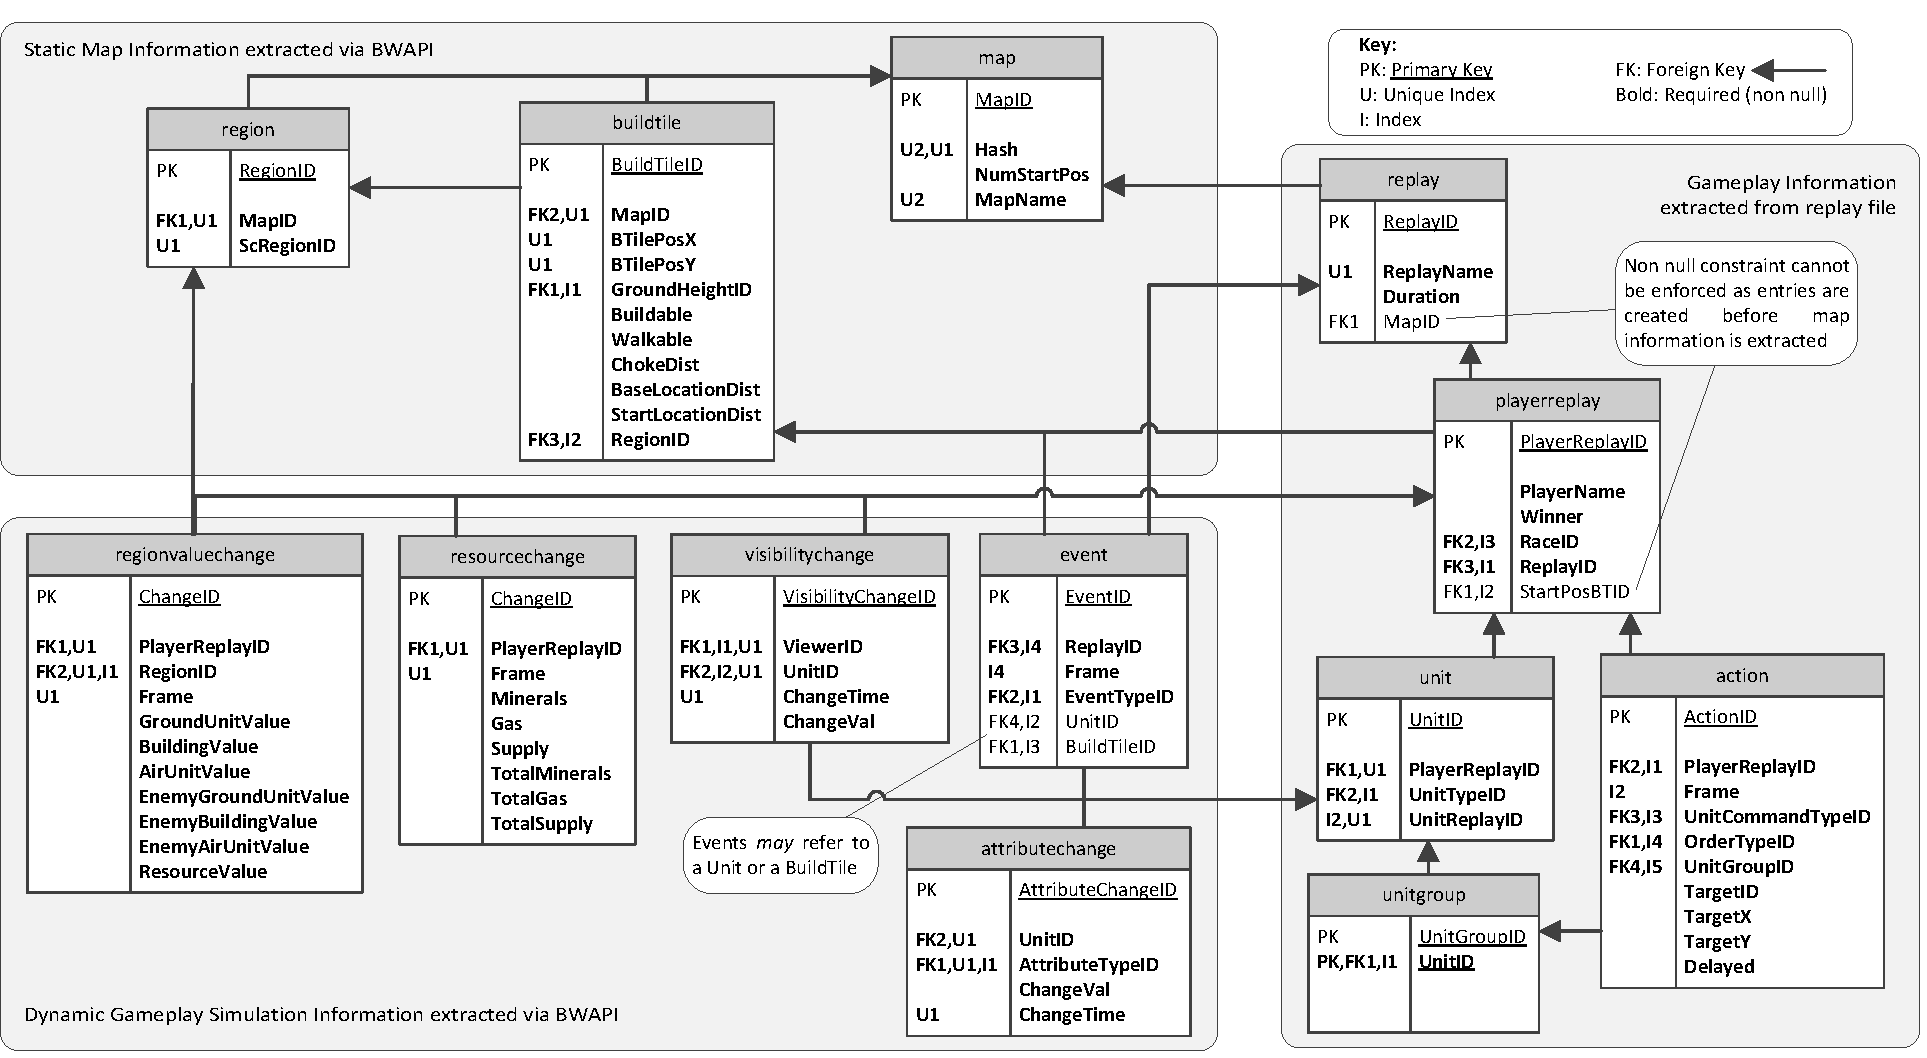
\includegraphics[width=\maxwidth]{figure/Robertson14DatabaseDiagram}
    \caption{Base de datos de partidas de StarCraft}
    \label{dataset}
\end{figure}



Una vez se tiene conocimiento del problema y un conjunto de datos, se
debe decidir qué datos y características van a ser usados y de qué
forma. El principal problema de este paso es conocer el conjunto de
datos del que se dispone, ya que usualmente no es extraído por los
investigadores.

Las características están sacadas casi en su totalidad directamente de
valores que proporciona la API que permite interactuar con StarCraft,
\emph{BWAPI}. Otros son datos derivados, como la distancia de un
jugador a la base más cercana, por ejemplo.

Las características que van a ser usados en este trabajo son,
principalmente, los recursos de cada jugador, sus batallones (que son
medidos de una manera determinada que se explican con más detalle más
adelante), sus construcciones, y los valores estimados de batallones y
contrucciones que tienen un jugador del otro. Además, también se tiene
en cuenta los recursos restantes del mapa que cada jugador estima que
quedan. Estas características quedan reflejadas en la figura
~\ref{datasetSeleccionado}.

\begin{figure}
    \centering
    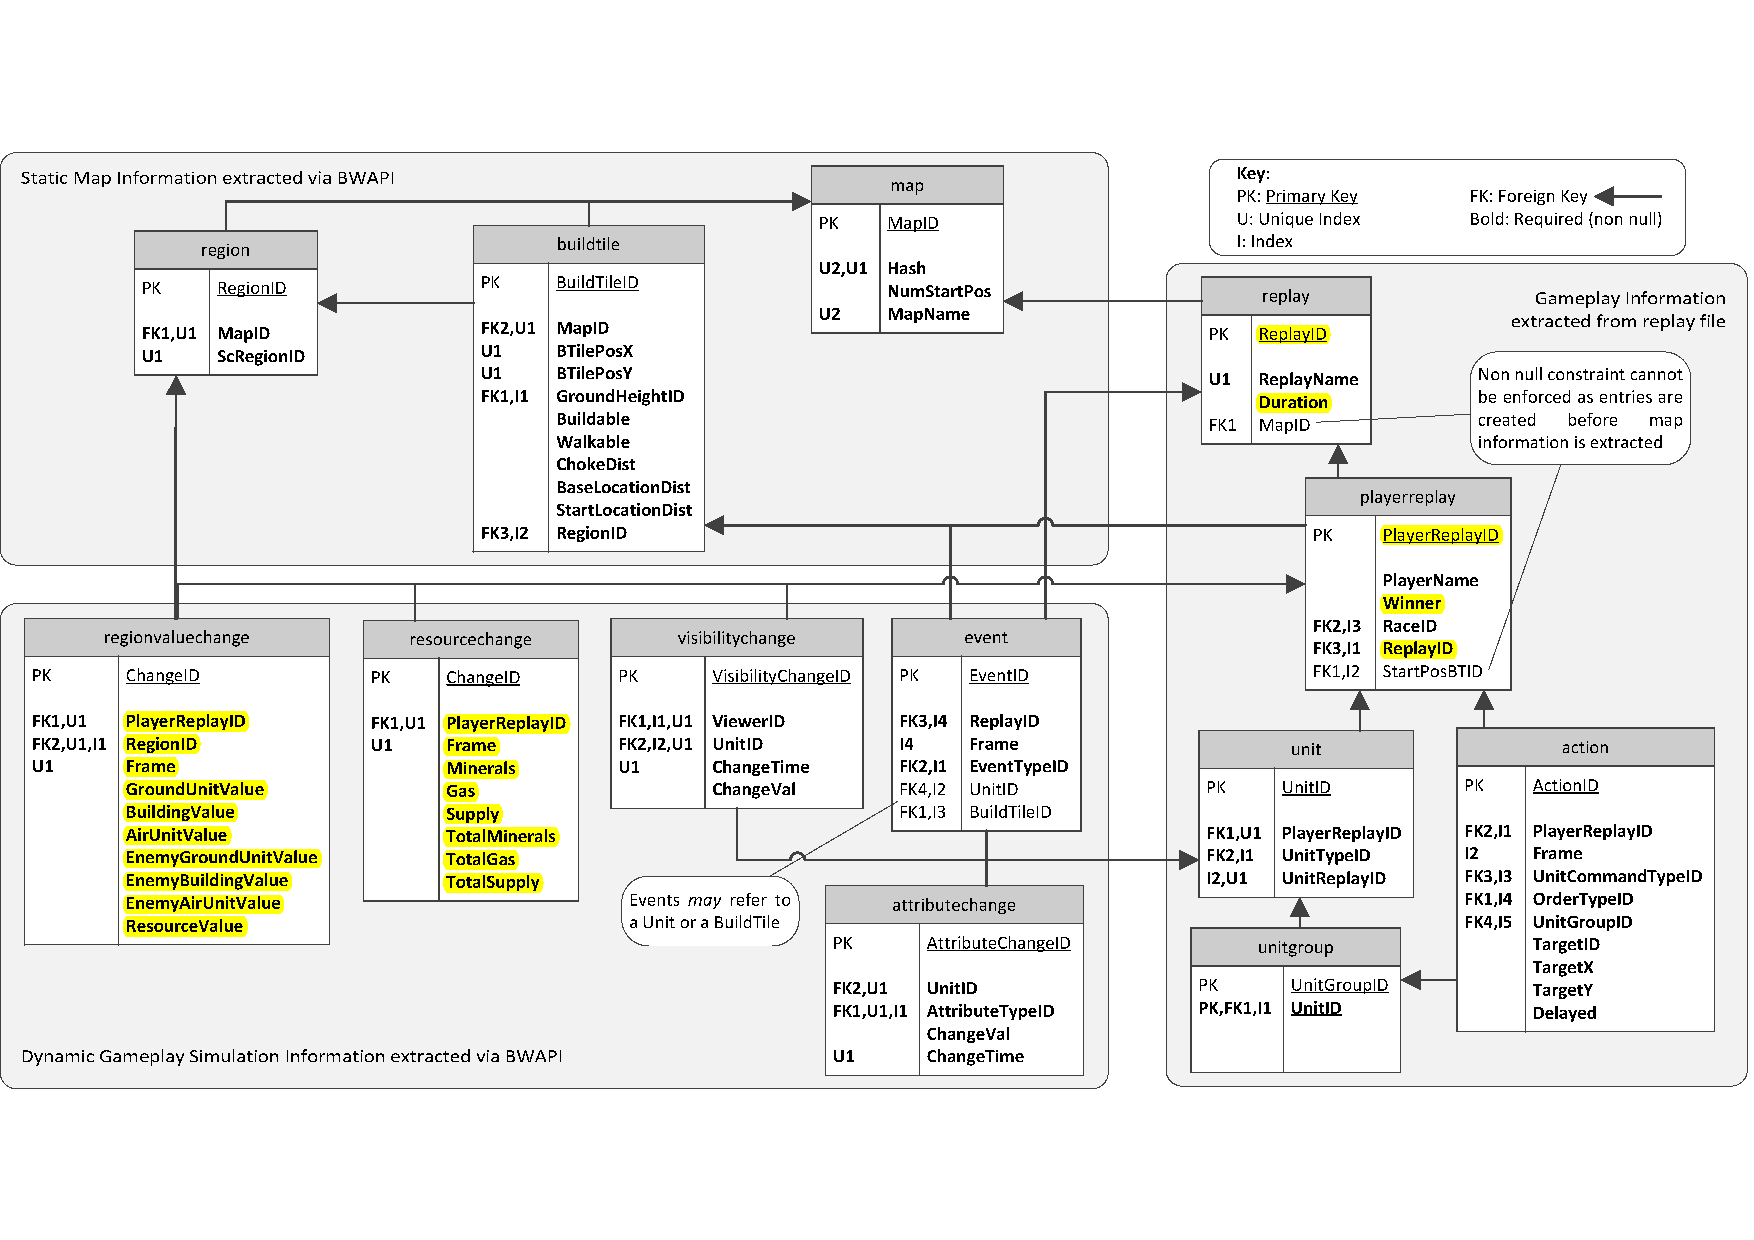
\includegraphics[width=\maxwidth]{figure/Robertson14DatabaseDiagramSeleccion}
    \caption{Características seleccionadas de las bases de datos}
    \label{datasetSeleccionado}
\end{figure}


Estas características son, según cada tabla:

\begin{itemize}
  \item replay: Esta tabla contiene datos asociados a cada partida.
  \begin{itemize}
    \item ReplayID: Identificador de cada partida.
    \item Duration: Duración (en frames) de cada partida. 15 frames equivalen a 1 segundo.
  \end{itemize}
  \item playerreplay: Esta tabla contiene datos asociados a un jugador en una partida.
  \begin{itemize}
    \item PlayerReplayID: Identificador de un jugador en una partida.
    \item ReplayID: Identificador de partida asociado.
    \item Winner: Ganador de cada partida.
  \end{itemize}
  \item resourcechange: Esta tabla contiene datos asociados a cambios en los recursos de un jugador.
  \begin{itemize}
    \item PlayerReplayID: Identificador del jugador que produce un cambio.
    \item Frame: Frame en el que se produce un cambio.
    \item Minerals: Cantidad de minerales que tiene un jugador en ese momento.
    \item Gas: Cantidad de gas que tiene un jugador en ese momento.
    \item Supply: Capacidad de carga del jugador.
    \item TotalMinerals: Cantidad total de minerales que ha obtenido un jugador, sin contar gastos.
    \item TotalGas: Cantidad total de gas que ha obtenido un jugador, sin contar gastos.
    \item TotalSupply: Capacidad que ha obtenido un jugador, sin contar gastos.
  \end{itemize}
  \item regionvaluechange: Esta tabla contiene datos asociados a cambios de un jugador en una región del mapa determinada. Cada \emph{value}, que llamaremos de aquí en adelante \emph{valor}, es la suma del precio de una unidad en Minerales y Gas.
  \begin{itemize}
    \item PlayerReplayID: Identificador del jugador que produce un cambio.
    \item RegionID: Identificador de la región del mapa donde se produce un cambio.
    \item Frame: Frame en el que se produce el cambio.
    \item GroundUnitValue: Valor de las unidades terrestres en esta región.
    \item BuildingValue: Valor de las construcciones en esta región.
    \item AirUnitValue: Valor de las unidades aéreas en esta región.
    \item EnemyGroundUnitValue: Valor de las unidades terrestres del enemigo en esta región. Este valor es estimado, sólo se conoce lo que el jugador puede ver del enemigo.
    \item EnemyBuildingValue: Valor de las contrucciones del enemigo en esta región. Este valor es estimado, sólo se conoce lo que el jugador puede ver del enemigo.
    \item EnemyAirUnitValue: Valor de las unidades aéreas del enemigo en esta región. Este valor es estimado, sólo se conoce lo que el jugador puede ver del enemigo.
    \item ResourceValue: Valor de los recursos en esta región. Este valor es estimado, sólo se conoce lo que el jugador puede ver del mapa. Si el jugador no conoce una zona, estima que los recursos restantes es la totalidad de lo disponible en la región.
  \end{itemize}
\end{itemize}

Una vez se ha decidido qué vamos a usar, hay que pasar al cómo. Esta fase es el \emph{preprocesamiento de los datos}, que es la fase donde se organizan los datos, se corrigen si hubiera datos perdidos o ruido... para poder abordar el problema a resolver.

\subsection{Preprocesamiento de datos}
\label{subsec:preprocesamiento}

\subsubsection{Análisis exploratorio de datos}
\label{subsubsec:exploratorio}

Lectura de datos

% <<readData>>=
% @

Histograma

% <<histograma>>=
% ggplot(data=metadata) +
% geom_bar(aes(x=ReplayID,y=Duration,fill=Duration), stat="identity") +
% geom_hline(yintercept = mean(metadata$Duration))
% print(mean(metadata$Duration))
% @


\chapter{Conclusiones} 

%%\chapter{Conclusiones y Trabajos Futuros}
%
%
%%\nocite{*}
%\bibliography{bibliografia/bibliografia}\addcontentsline{toc}{chapter}{Bibliografía}
%\bibliographystyle{miunsrturl}
%
%\appendix
%\input{apendices/manual_usuario/manual_usuario}
%%\input{apendices/paper/paper}
%\input{glosario/entradas_glosario}
% \addcontentsline{toc}{chapter}{Glosario}
% \printglossary
\chapter*{}
\thispagestyle{empty}

\bibliography{bibliografia}{}
\bibliographystyle{plain}

\end{document}
